\section{Introduction}

\vspace{-0.em}
\begin{figure}[t]
    \centering
    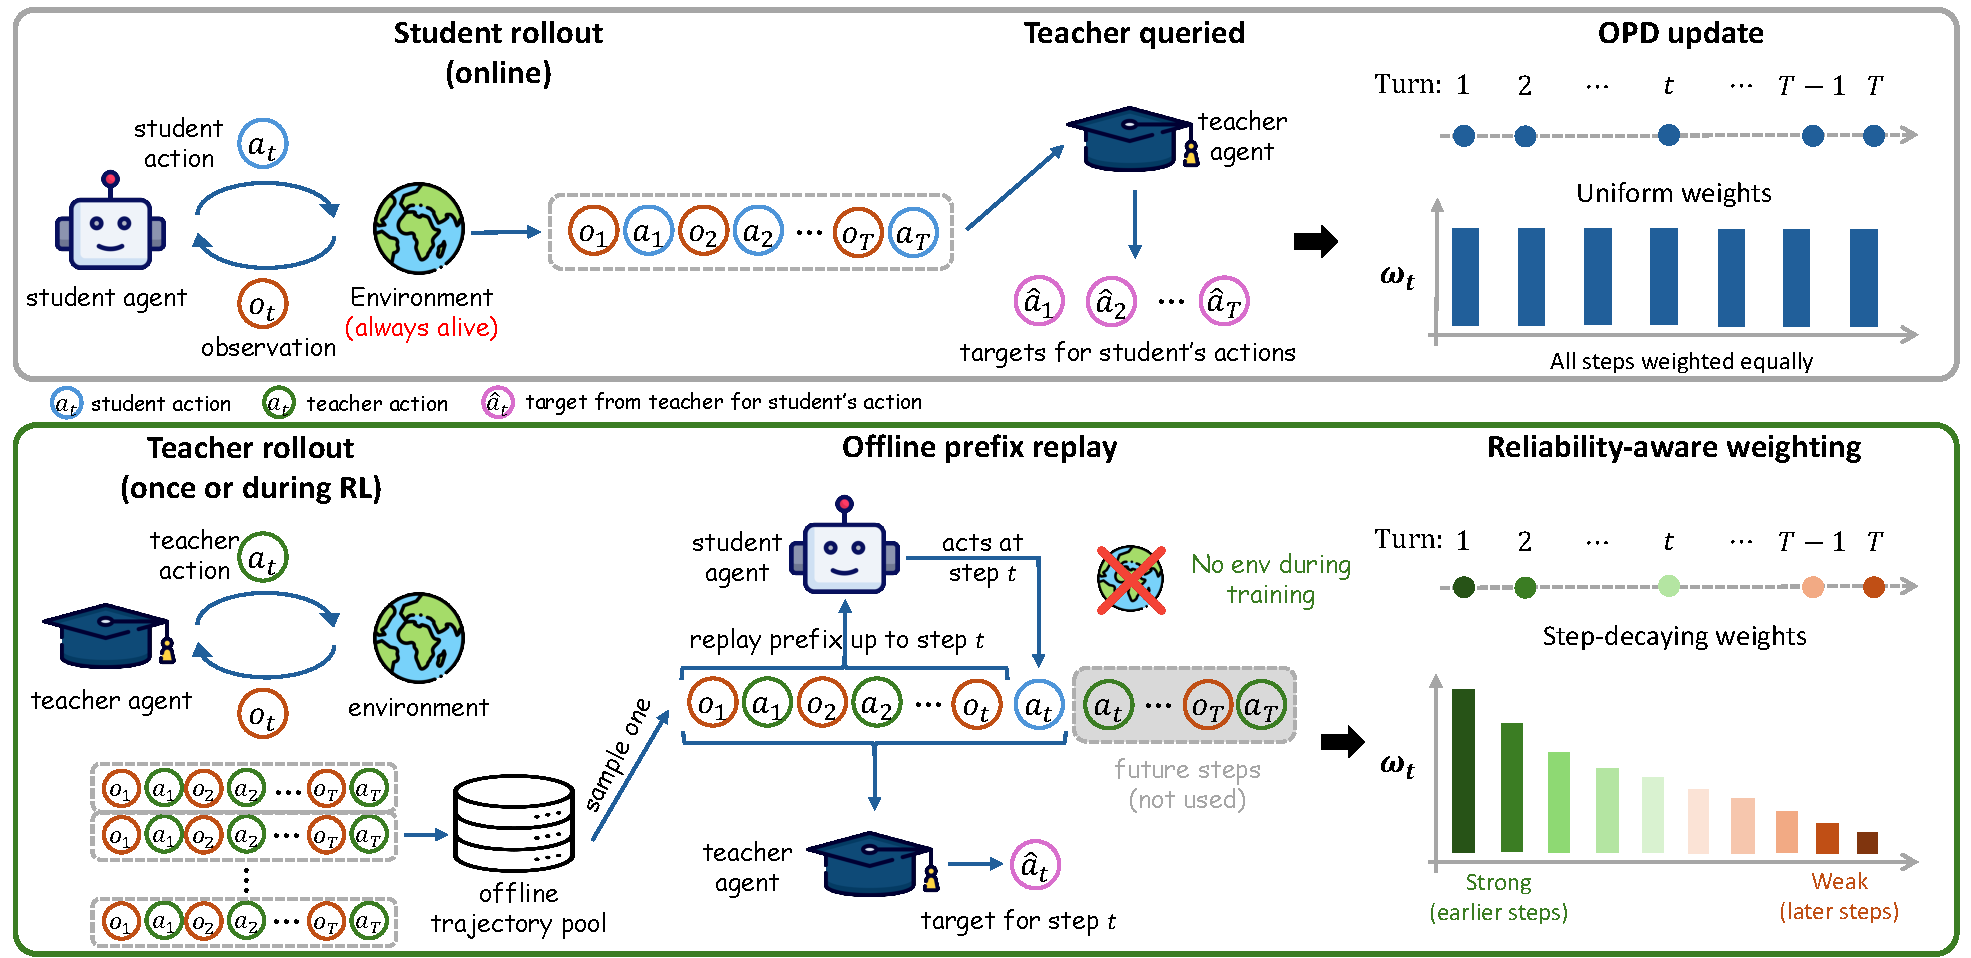
\includegraphics[width=0.99\linewidth]{figs/aopd.pdf}
  \caption[]{\textbf{Comparison between OPD and ReOPD for agentic tasks}. \textbf{Up:} OPD with online environment. The environment is always alive during training. And all steps equally contribute to the loss. \textbf{Down:} ReOPD with offline environment. The environment is only alive for collecting the teacher's trajectories, which can happen during the training of the teacher agent by using RL, like GRPO. Afterwards, the environment is not needed for the training of the student agent. The earlier steps contribute more to the loss.}
  \label{fig:overview}
  \vspace{-0mm}
\end{figure}


\vspace{-0.em}
\begin{figure}[t]
    \centering
    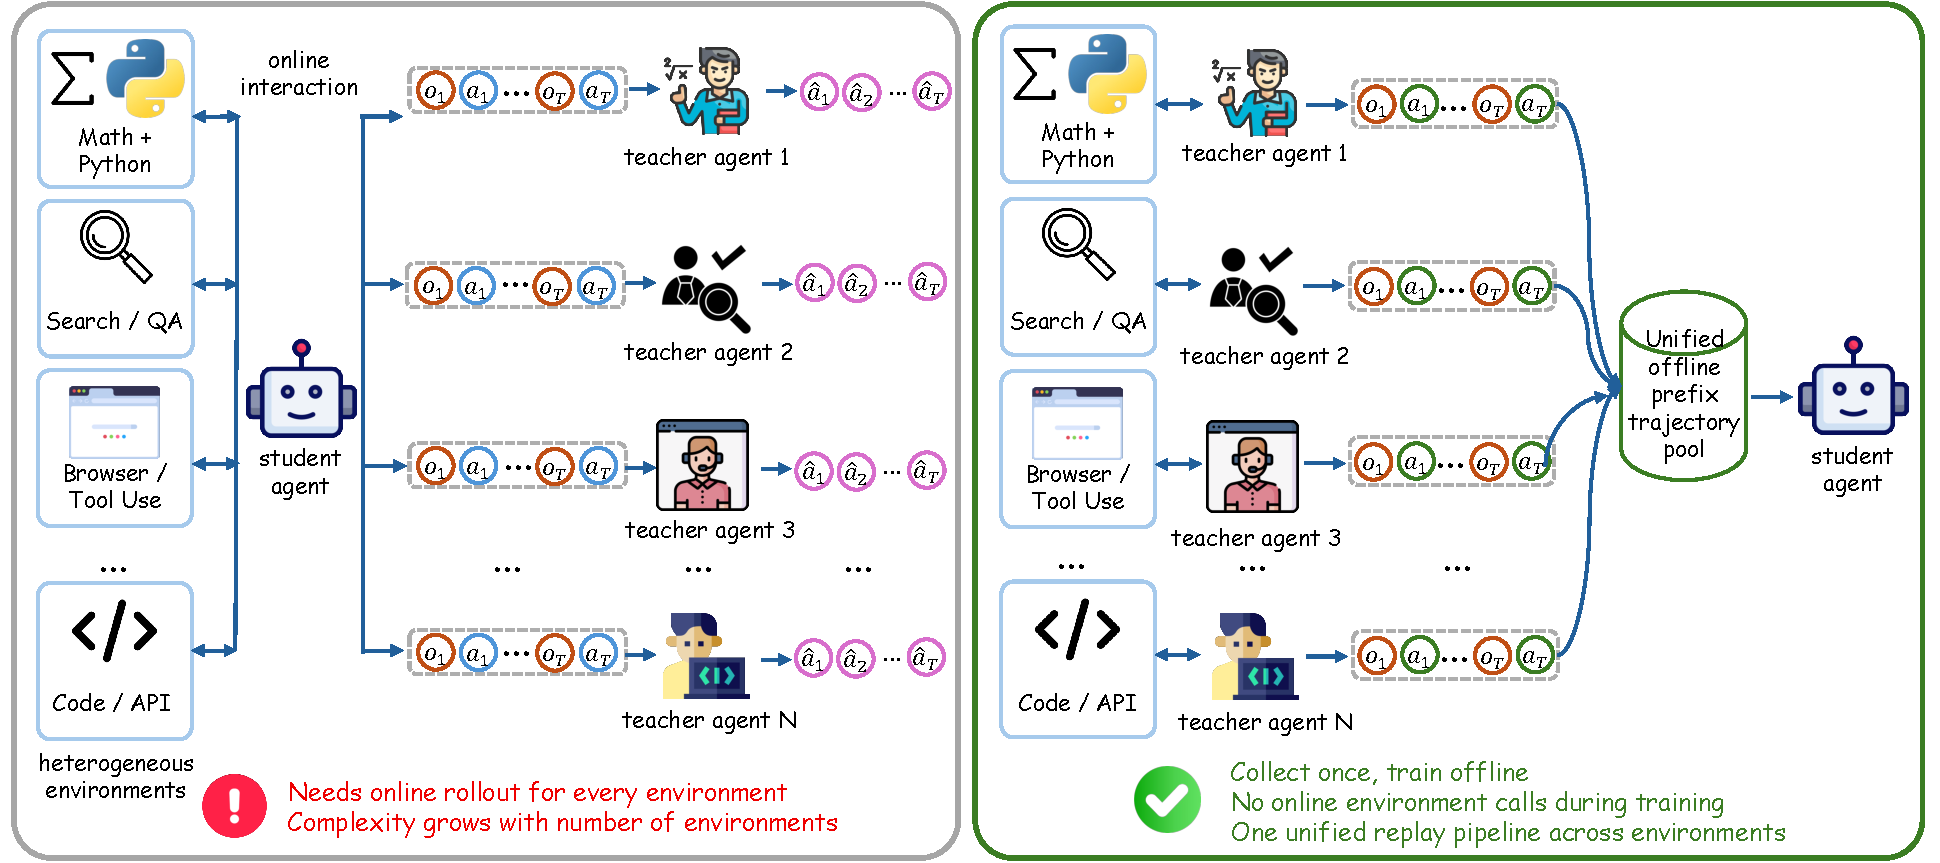
\includegraphics[width=0.99\linewidth]{figs/aopd_multi_envs.pdf}
  \caption[]{\textbf{Training a shared student agent on multiple heterogeneous environments with OPD and ReOPD.} \textbf{Left:} With an increasing number of environments, the operational complexity grows for OPD due to the heavy deployment of the environments. \textbf{Right:} ReOPD doesn't require the deployment of all environments at the same time. The teacher's trajectories can be collected separately for different environments, and then be merged into a unified pool for the later training of the student agent without any online environment.}
  \label{fig:overview_multi_envs}
  \vspace{-0mm}
\end{figure}

Reinforcement learning (RL) has become a central tool for eliciting strong
reasoning and agentic behavior from large language models (LLMs). Policy-gradient
methods such as PPO~\citep{schulman2017proximal} and GRPO~\citep{shao2024deepseekmath},
together with verifiable rewards, drive much of the recent progress on
mathematical reasoning and tool use~\citep{deepseekai2025deepseekr1incentivizingreasoningcapability,yu2025dapo}.
A defining property of RL is that it is \emph{on-policy}: the model is trained on
trajectories sampled from itself, so it learns to recover from its own mistakes
rather than from mistakes made by some other distribution. However, RL supervision
is sparse: a scalar reward conveys only a few bits per episode, regardless of how
many tokens were generated~\citep{thinkingmachines2025onpolicy}, which makes it
sample-inefficient, particularly for small models.

Knowledge distillation offers a much denser learning signal by training a student
to imitate a stronger teacher~\citep{hinton2015distilling,kim2016sequence}. The
standard recipe is \emph{off-policy}: the student is supervised on teacher-generated
trajectories via sequence-level distillation or supervised fine-tuning. While
data-efficient, off-policy distillation trains the student on prefixes visited by
the \emph{teacher}, not by the student itself. When the student later makes an early
mistake the teacher would not, it drifts into prefixes never seen during training,
and errors compound over the sequence~\citep{ross2011reduction,ranzato2016sequence}.
\emph{On-policy distillation} (OPD) addresses this by sampling prefixes from the
student while still distilling against the teacher's per-token
distribution~\citep{gu2024minillm,agarwal2024gkd,thinkingmachines2025onpolicy},
combining the relevance of on-policy data with the density of teacher supervision.

These ideas were largely developed for single-turn generation. Modern LLMs,
however, increasingly tackle \emph{agentic tasks}, operating as \emph{agents} that
interact with external environments over multiple turns, interleaving actions such as code execution,
retrieval, or search engine calls with the environment
feedback~\citep{yao2022react,schick2023toolformer,nakano2021webgpt,jin2025search}.
Coupling this multi-turn structure with teacher distillation gives \emph{multi-turn OPD}:
at each turn, the student rolls into a history, and the teacher supplies an
improvement target. Realized online, this is expensive -- every update must roll the student through the environment and query the teacher afresh at each visited
history, incurring environment-interaction and teacher-inference cost at every
step. A far more efficient alternative -- \emph{prefix replay} -- reuses trajectories the teacher has already
produced (Figure~\ref{fig:overview}): the student is rolled in on a teacher-recorded prefix and generates its
own action at the evaluated step, the prefix and its observations are taken from the
trace instead of executing actions, and the teacher supplies the per-step target.
The student thus stays on-policy at the supervised step -- but not along the
teacher-forced prefix itself -- while the environment is never queried; ReOPD therefore
trades a fully on-policy roll-in for reusability, a tension we make precise as a
two-sided distribution shift in Section~\ref{sec:formulation}. Crucially, such trajectories are not an added cost: when the teacher
is itself trained with RL, its on-policy rollouts are already collected during
training, so the prefix pool comes for free and distillation requires no extra
environment interaction. This decoupling compounds when a single student must learn
from several heterogeneous environments: instead of deploying all of them
simultaneously, ReOPD collects each teacher's trajectories separately and merges them
into one offline pool for student training (Figure~\ref{fig:overview_multi_envs}).
Figure~\ref{fig:overall} illustrates the payoff: ReOPD retains the
accuracy benefits of OPD while sharply reducing per-step training time and tool
calls. This motivates the question we study:
\emph{How should multi-turn OPD be done when the environment is
replaced by replayed teacher prefixes rather than fresh online rollouts?} In
this setting, prefixes act as implicit states and multi-turn generation induces
an implicit trajectory distribution over them.

Training offline in this way does not remove the temporal structure of multi-turn
learning, and we identify a \emph{prefix trap} with two layers. The first is
\emph{temporal}: prefix errors compound across steps, so the problem stays
sequential. The second is \emph{distributional} -- a \emph{two-sided shift}:
Making prefixes fully student-on-policy keeps them relevant to the student (a
student occupancy shift) but can query the teacher where its condition is no
longer a trustworthy target (a teacher reliability shift). A simple decomposition
bounds the gap to an ideal interactive objective by exactly these two terms.
Multi-turn OPD is therefore not just ``make distillation on-policy'' but
\emph{reliability-aware prefix distribution design}: choosing, at each step, an
effective prefix distribution between student and teacher occupancies; a concrete
sampling or weighting schedule is an implementation.

This view predicts a regime-aware outcome that our experiments confirm: OPD is already
strong when the teacher stays reliable on student-induced histories, whereas leaning on teacher trajectories
and down-weighting high-shift late steps wins when the teacher--student gap is large, even though it is less
on-policy.

\paragraph{Contributions.} Our contributions are as follows.
\begin{itemize}[leftmargin=1.5em,itemsep=2pt,topsep=2pt]
  \item We study \emph{efficient} Replayed-Prefix On-Policy Distillation that reuses a
  fixed pool of offline teacher trajectories, and surface the \emph{prefix trap},
  separating its temporal (compounding-error) and distributional (two-sided shift)
  layers.
  \item We formulate multi-turn OPD as a two-sided distribution-shift problem and
  derive a bound that decomposes the objective gap into a student
  occupancy-mismatch term and a teacher reliability term, showing why fully
  student-on-policy distillation is not automatically optimal.
  \item We recast multi-turn OPD as a reliability-aware prefix distribution design, with
  a geometric bridge between student and teacher occupancies, and show that a simple
  step-decay schedule -- applied by sampling prefixes -- is a practical implementation
  of the resulting effective distribution.
  \item We validate the resulting method, \emph{Replayed-Prefix On-Policy Distillation} (ReOPD), on mathematical reasoning and search environments,
  across single- and multi-environment settings and teacher and student models of varying
  scale. ReOPD improves over off-policy distillation (SFT) where reported; relative to
  strong on-policy OPD, and consistent with our two-regime analysis, it improves on
  mathematical reasoning when the teacher-student gap is wide and essentially matches
  OPD when the teacher is already reliable on the student histories (search/QA).
\end{itemize}
